\section{Probabilistic graphical models}
\begin{itemize}
	\item It is often beneficial to visualize a probabilistic model as a diagram, which we call \textit{(probabilistic) graphical models}. 
	\item They are good for:
	\begin{itemize}
		\item causal reasoning/modeling
		\item calculating inference and conditional distributions efficiently 
		\item Designing and communicating statistical model
		\item Encoding (conditional) independence relations
	\end{itemize} 
	\item Note that there are often multiple ways to express the same probability distribution. For example, take a joint distribution $p(A,B,C)$, which we can either write as $p(A,B,C)=p(A)p(B|A)p(C|A,B)$ (see Figure~\ref{fig:graphical_models_example_1}) or $p(A,B,C)=p(C)p(A|C)p(B|A,C)$ (see Figure~\ref{fig:graphical_models_example_2}). Nevertheless, what we interested in the end is the graphical representation with the least number of edges, as e.g. if $A$ and $B$ are independent (conditionally on $C$), we can drop the edge between those.
	\begin{figure}[ht!]
		\centering
		\begin{subfigure}{0.4\textwidth}
			\centering
			\tikz{ %
				\node[latent] (A) {$A$} ; %
				\node[latent, right=of A] (B) {$B$} ; %
				\node[latent, below=of B] (C) {$C$} ; %
				
				\edge{A}{B};
				\edge{A}{C};
				\edge{B}{C};
			}
			\caption{$p(A,B,C)=p(A)p(B|A)p(C|A,B)$}
			\label{fig:graphical_models_example_1}
		\end{subfigure}
		\hspace{10mm}
		\begin{subfigure}{0.4\textwidth}
			\centering
			\tikz{ %
				\node[latent] (A) {$A$} ; %
				\node[latent, right=of A] (B) {$B$} ; %
				\node[latent, below=of B] (C) {$C$} ; %
				
				\edge{A}{B};
				\edge{C}{A};
				\edge{C}{B};
			}
			\caption{$p(A,B,C)=p(C)p(A|C)p(B|A,C)$}
			\label{fig:graphical_models_example_2}
		\end{subfigure}
		\caption{Two different graphical models (here Bayesian Networks) for the same joint distribution $p(A,B,C)$.}
	\end{figure}
	\item We distinguish between directed acyclic graphs, which we call \textit{Bayesian networks} (BN), and undirected graphs, which are \textit{Markov Random Fields} (MRF)
\end{itemize}

\subsection{Bayesian Networks}
\begin{itemize}
	\item There is a simple way for creating a Bayesian network for a given statistical model.
	\begin{enumerate}
		\item Determine the ordering of the variables (``\textit{topological ordering}'')
		\item In this ordering, call the parents of the random variable $X_i$: $\text{pa}_i$, or $\text{pa}(X_i)$ which is a subset of variables with lower ordering: $\text{pa}_i \subseteq \left\{X_1,...,X_{i-1}\right\}$. The joint probability distribution can be written as:
		$$p(X_1,...,X_M) = \prod_{i=1}$$
		\item In the graphical model, draw an edge from $X_i$ to $X_j$ if $j\in \text{pa}_i$
	\end{enumerate}
	\item \underline{Example}: (first-order) Markov Chain
	\begin{itemize}
		\item The joint probability distribution of a Markov Chain can be expressed by:
		$$p(X_1,...,X_M)=p(X_1)\cdot \prod_{i=2}^{M} p(X_i|X_{i-1})$$
		\item The corresponding Bayesian Network looks as follows:
		\begin{figure}[ht!]
			\centering
			\tikz{ %
				\node[obs] (x1) {$X_1$} ; %
				\node[obs, right=of x1] (x2) {$X_2$} ; %
				\node[obs, right=of x2] (x3) {$X_3$} ; %
				\node[const, right=of x3] (xetc1) { \hspace{2mm}...\hspace{2mm} } ; %
				\node[obs, right=of xetc1] (xM) {$X_M$} ; %
				
				\edge{x1}{x2};
				\edge{x2}{x3};
				\edge{x3}{xetc1};
				\edge{xetc1}{xM};
			}
		\end{figure}
		where the filling expresses that $X_i$ is an observed variable.
	\end{itemize}
	\item \underline{Example}: Regression
	\begin{itemize}
		\item Suppose we a simple regression problem where we want to learn parameters $W$ to predict targets $T$ from input $X$. We further assume that we know our sensory noise $\sigma^2$, and have a prior with hyperparameters $\alpha$.
		\item We can express this in the following graphical model:
		\begin{figure}[ht!]
			\centering
			\tikz{ %
				\node[obs] (x) {$X_n$} ; %
				\node[obs, right=of x] (t) {$T_n$} ; %
				\plate{xt}{(x)(t)}{$n=1,...,N$};
				
				\node[latent, above=of t] (w) {$W$} ; %
				\node[const, left=of w] (alpha) {$\alpha$} ; %
				\node[const, right=of t] (sigma) {$\sigma^2$} ; %
				
				\edge{x}{t};
				\edge{w}{t};
				\edge{alpha}{w};
				\edge{sigma}{t};
			}
		\end{figure}
		which represents the probability distribution
		$$p(W, \left\{T_n\right\}, \left\{X_n\right\}|\alpha, \sigma^2)p(W|\alpha)\prod_{n=1}^{N} \left[p(T_n|X_n, W, \sigma^2)p(X_n)\right]$$
		Note that in the graphical model, $\alpha$ and $\sigma^2$ are assumed to be fixed an known, and the ``plate'' can be interpreted as copying the content $N$ times (i.e. we have $N$ $X_i$ and $T_i$ variables with the same edges).
		
		Also, if desired, we could have used a constant for the data points $X_i$ as well as these are often assumed to be fixed.
		\item If we also want to express the predictive distribution $p(T^{*}|X^{*},W, \left\{T_n\right\}, \left\{X_n\right\},\alpha, \sigma^2)$, we can extend our model as follows:
		\begin{figure}[ht!]
			\centering
			\tikz{ %
				\node[obs] (x) {$X_n$} ; %
				\node[obs, right=of x] (t) {$T_n$} ; %
				\plate{xt}{(x)(t)}{$n=1,...,N$};
				
				\node[latent, above=of t] (w) {$W$} ; %
				\node[const, left=of w] (alpha) {$\alpha$} ; %
				\node[const, right=of t] (sigma) {$\sigma^2$} ; %
				
				\node[latent, right=of w] (tstar) {$T^{*}$} ; %
				\node[obs, right=of tstar] (xstar) {$X^{*}$} ; %
				
				
				\edge{x}{t};
				\edge{w}{t};
				\edge{w}{tstar};
				\edge{xstar}{tstar};
				\edge{alpha}{w};
				\edge{sigma}{t};
				\edge{sigma}{tstar};
			}
		\end{figure}
	\end{itemize}
\end{itemize}
\subsubsection{Conditional independence and D-separation}
\begin{itemize}
	\item A useful property of graphical models is that we can easily study the independence relations between random variables in our model. 
	\item We call $X$ and $Y$ being independent iff $p(X,Y)=p(X)p(Y)$. The notation for this is $X\independent Y$
	\item $X$ is \textit{conditionally} independent of $Y$ given $Z$ if $p(X,Y|Z)=p(X|Z)p(Y|Z)$. The notation for this is $X\independent Y|Z$. Note that if $X$ and $Y$ are generally independent, we can also write $X\independent Y|\emptyset$
	\item For proving/testing conditional independence, we can use \textbf{d-separation}. Supposed $A$, $B$, $C$ are sets of variables. If $A$ is d-separated from $B$ given $C$, then $p(X_A,X_B|X_C)=p(X_A|X_C)p(X_B|X_C)$, which we can also write as $A\perp B|C\implies X_A\independent X_B|X_C$ 
	\item Note that the other way round, $X_A\independent X_B|X_C\not\implies A\perp B|C $ is not always valid (but mostly) as we will show in a later example. Hence, if $A$ and $B$ are not d-separated, it does not necessarily mean that $X_A$ and $X_B$ are not conditional independent.
	
	\item The algorithm can be summarized as follows:
	\begin{tcolorbox}[colback=white!80!gray,colframe=gray!75!black,title=D-separation]
		Given the sets of variables $A$, $B$, $C$:
		\begin{enumerate}
			\item Consider all paths (sequence of nodes, connected by edges,  s.t. no node repeats) between any node in $A$ and any node in $B$
			\item Mark a path as \underline{blocked} by $C$ if
			\begin{enumerate}
				\item It contains a collider $...\rightarrow u \leftarrow ...$ such that $u$ is not an ancestor of a node in $C$
				\item It contains a non-collider $...\rightarrow u$, $...\rightarrow u \rightarrow ...$, $...\leftarrow u \rightarrow ...$ such that $u$ is in $C$
			\end{enumerate}
			\item If all paths are marked as blocked by $C$, then $A$ is d-separated from $B$ given $C$
		\end{enumerate}
	\end{tcolorbox}	
	\item \underline{Examples}: 
	\begin{itemize}
		\item Consider the following graphical model:
		\begin{figure}[ht!]
			\centering
			\tikz{ %
				\node[latent] (xA) {$X_A$} ; %
				\node[latent, right=of xA] (xB) {$X_B$} ; %
				\node[latent, below=of xB] (xC) {$X_C$} ; %
				
				\edge{xC}{xA};
				\edge{xC}{xB};
			}
		\end{figure}
	
		$A$ is d-separated from $B$ given $C$ as the only way from $B$ to $A$ is through $X_C$, and it represents a non-collider: $X_A\independent X_B|X_C$.
		
		Note that $A$ is not d-separated from $B$ given $\emptyset$ because $X_C$ is then neither a non-collider nor a collider.
		\item Consider the following graphical model:
		\begin{figure}[ht!]
			\centering
			\tikz{ %
				\node[latent] (xA) {$X_A$} ; %
				\node[latent, right=of xA] (xC) {$X_C$} ; %
				\node[latent, right=of xC] (xB) {$X_B$} ; %
				
				\edge{xA}{xC};
				\edge{xC}{xB};
			}
		\end{figure}
	
		Similarly to the previous model, $A$ is d-separated from $B$ given $C$ as the only way from $B$ to $A$ is through $X_C$, and it represents a non-collider: $X_A\independent X_B|X_C$.
		
		However, here we can show a special case where conditional independence does not imply d-separation. Suppose that we model $p(C|A)=\delta_{C,A}$, hence being a deterministic mapping. Now, $C\independent B|A$ holds because if we know $A$, we know $C$ for certain. Nevertheless, the d-separation is not valid because there is a direct path from $C$ to $B$! 
		
		\item Consider the following graphical model:
		\begin{figure}[ht!]
			\centering
			\tikz{ %
				\node[latent] (xA) {$X_A$} ; %
				\node[latent, right=of xA] (xC) {$X_C$} ; %
				\node[latent, above=of xC] (xB) {$X_B$} ; %
				\node[const, right=of xC] (xetc) {\hspace{2mm}...\hspace{2mm} } ; %
				\node[latent, right=of xetc] (xD) {$X_D$} ; %
				
				\edge{xA}{xC};
				\edge{xB}{xC};
				\edge{xC}{xetc};
				\edge{xetc}{xD};
			}
		\end{figure}
	
		$A$ is d-separated from $B$ given the empty set as $X_C$ represents a collider which is not in the empty set: $X_A\independent X_B|\emptyset$.
		
		$A$ is \textit{not} d-separated from $B$ given $C$ because $X_C$ is then not a collider anymore: $A\not\perp B|C$.
		
		$A$ is \textit{not} d-separated from $B$ given $D$ because $X_C$ is an ancestor of a node in $D$, and hence, not a collider: $A\not\perp B|D$.
	\end{itemize}
\end{itemize}
\subsubsection{Markov blanket}
\begin{itemize}
	\item A Markov blanket of a variable $X_i$ is defined as the set of variables which are the parents, children or children's parents of $X_i$, except $X_i$ itself:
	$$\text{MB}(X_i)=\text{pa}_i \cup \text{ch}_i \cup \left(\text{pa}_{\text{ch}_i}\setminus i\right)$$
	\item The important property of the Markov blanket is that, for a random variable $X_i$ in any BN, given its Markov blanket $\text{MB}(X_i)$, it is conditionally independent of the rest of the graph:
	$$p\left(X_i|X_{\text{MB}(X_i)}, X_{\text{res}}\right) = p\left(X_i|X_{\text{MB}(X_i)}\right)$$
	\item \underline{Example}: For the graphical model of the regression problem, the Markov blanket of $T^{*}$ is $\text{MB}(T^{*})=\left\{X^{*}, W\right\}$. This result is intuitive as once we have trained our model, we do not need to revisit our data or our prior over $W$. Note that $\sigma^2$ is a constant, and hence not in the Markov blanket.
\end{itemize}
\subsection{Markov Random Fields}
\begin{itemize}
	\item A Markov Random Field is a undirected graphical models. Hence, our model consists now of two parts: the undirected graph $G$, and so called (maximum) cliques potentials $\left\{\psi_A\right\}$
	\item A clique in a undirected graph $G$ is a fully connected subset of nodes. Hence, also single nodes are considered as a clique.
	\begin{itemize}
		\item A clique is \textit{maximal} if there is no clique that strictly contains it, i.e. we cannot add another node to the clique which is fully connected to all others. 
		\item \underline{Example}: Consider the following graphical model:
		\begin{figure}[ht!]
			\centering
			\tikz{ %
				\node[latent] (xA) {$X_A$} ; %
				\node[latent, right=of xA] (xB) {$X_B$} ; %
				\node[latent, below=of xA] (xC) {$X_C$} ; %
				\node[latent, right=of xC] (xD) {$X_D$} ; %
				\node[latent, right=of xD] (xE) {$X_E$} ; %
				\node[latent, left=of xA] (xF) {$X_F$} ; %
				
				\edge[-]{xA}{xC};
				\edge[-]{xA}{xB};
				\edge[-]{xC}{xD};
				\edge[-]{xB}{xD};
				\edge[-]{xB}{xE};
				\edge[-]{xE}{xD};
			}
		\end{figure}
	
		Then our maximum cliques are $\{X_A,X_C\}, \{X_A, X_B\}, \{X_C,X_D\},\{X_B,X_D,X_E\},\{X_F\}$
	\end{itemize}
	\item We can now write our joint probability distribution in terms of the maximum cliques $\left\{\psi_A\right\}$:$$p(x_1,...,x_N)=\frac{1}{Z}\prod_A \psi_A(x_A)$$
	Note that we now need a normalization constant $Z$ which we did not need for Bayesian networks. The reason for this is that clique potentials might not be normalized. The only requirement for them is to be positive for any $x_A$, and are thus often modeled by a energy function $\psi_A(x_A) = \exp(f(x_A))$ (hence the name \textit{potential})
	\item For the previous example, our probability distribution can be now written as:
	$$p(x_A,...,x_E)=\frac{1}{Z}\psi_{A,B}(x_A,x_B)\psi_{A,C}(x_A,x_C)\psi_{C,D}(x_C,x_D)\psi_{B,D,E}(x_B,x_D,x_E)\psi_{F}(x_F)$$
	where $Z=\sum_{x_A}\sum_{x_B}...\sum_{x_F}\psi_{A,B}(x_A,x_B)\psi_{A,C}(x_A,x_C)...\psi_{F}(x_F)$
	\item One disadvantage of undirected graphs, as we can see here, is that we need to calculate $Z$ which grows exponentially with the number of variables.
	\item We can also define the properties of separation and Markov blanket for undirected graphs:
	\begin{description}
		\item[Separation] similarly to d-separation in BNs, two subsets of nodes $A$ and $B$ are \underline{separated} given $C$ if each path between a node in $A$ and a node in $B$ passes through (at least one) node $C$:
		$$A\perp B|C\implies X_A\independent X_B|X_C$$
		\item[Markov blanket] The Markov blanket for MRFs is defined as the neighbors of $i$, i.e. the nodes adjacent to $i$. In the previous example, the Markov blanket of $X_B$ is: $\text{MB}(X_B) = \{X_A,X_D,X_E\}$
	\end{description}
\end{itemize}
\subsubsection{Converting Bayesian network to MRFs}
\begin{itemize}
	\item Sometimes it is the case that we want to represent a same statistical model which we have as a Bayesian network, also as a MRF. This is the case when we want to apply algorithms which are generally defined for undirected graphs (e.g. sum-product)
	\item The \textit{Hammersley-Clifford} theorem states that any strictly positive, joint distribution $p(\bm{X})\ge 0$ can be represented as a MRF. Hence, we can also do it with any Bayesian network
	\item Nevertheless, note that by converting a BN to a MRF, some properties/information might be lost, such as (conditional) independence relations. 
	\item \underline{Examples}:
	\begin{itemize}
		\item Consider a first-order Markov chain:
		\begin{figure}[ht!]
			\centering
			\begin{subfigure}{0.46\textwidth}
				\centering
				\tikz{ %
					\node[obs] (x1) {$x_1$} ; %
					\node[obs, right=of x1] (x2) {$x_2$} ; %
					\node[const, right=of x2] (xetc) {\hspace{2mm}...\hspace{2mm} } ; %
					\node[obs, right=of xetc] (xM) {$x_M$} ; %
					
					\edge{x1}{x2};
					\edge{x2}{xetc};
					\edge{xetc}{xM};
				}
				\caption{BN}
			\end{subfigure}
			\hspace{5mm}
			\begin{subfigure}{0.46\textwidth}
				\centering
				\tikz{ %
					\node[obs] (x1) {$x_1$} ; %
					\node[obs, right=of x1] (x2) {$x_2$} ; %
					\node[const, right=of x2] (xetc) {\hspace{2mm}...\hspace{2mm} } ; %
					\node[obs, right=of xetc] (xM) {$x_M$} ; %
					
					\edge[-]{x1}{x2};
					\edge[-]{x2}{xetc};
					\edge[-]{xetc}{xM};
				}
				\caption{MRF}
			\end{subfigure}
		\end{figure}
	
		As Bayesian network, we can represent it with the probability density function $p(x_1)\prod_{i=2}^{M}p(x_i|x_{i-1})$.
		
		In the case of the MRF, we have $\frac{1}{Z}\prod_{i=2}^{M}\psi_{i-1,i}(x_{i-1},x_i)$. Note that the prior $\psi_1(x_1)$ is integrated in $\psi_{1,2}(x_1,x_2)$ as the clique potentials are more flexible than the conditional probabilities in Bayesian networks.
		
		\item Consider the following Bayesian network:
		\begin{figure}[ht!]
			\centering
			\begin{subfigure}{0.25\textwidth}
				\centering
				\tikz{ %
					\node[latent] (xA) {$X_A$} ; %
					\node[latent, right=of xA] (xC) {$X_C$} ; %
					\node[latent, below=of xC] (xB) {$X_B$} ; %
					\node[latent, below=of xA] (xD) {$X_D$} ; %
					
					\edge{xA}{xC};
					\edge{xB}{xC};
					\edge{xD}{xA};
				}
				\caption{BN}
			\end{subfigure}
			\hspace{5mm}
			\begin{subfigure}{0.25\textwidth}
				\centering
				\tikz{ %
					\node[latent] (xA) {$X_A$} ; %
					\node[latent, right=of xA] (xC) {$X_C$} ; %
					\node[latent, below=of xC] (xB) {$X_B$} ; %
					\node[latent, below=of xA] (xD) {$X_D$} ; %
					
					\edge[-]{xA}{xC};
					\edge[-]{xB}{xC};
					\edge[-]{xD}{xA};
				}
				\caption{(Potential) MRF}
				\label{fig:graphical_models_BN_to_MRF_2}
			\end{subfigure}
			\hspace{5mm}
			\begin{subfigure}{0.25\textwidth}
				\centering
				\tikz{ %
					\node[latent] (xA) {$X_A$} ; %
					\node[latent, right=of xA] (xC) {$X_C$} ; %
					\node[latent, below=of xC] (xB) {$X_B$} ; %
					\node[latent, below=of xA] (xD) {$X_D$} ; %
					
					\edge[-]{xA}{xC};
					\edge[-]{xB}{xC};
					\edge[-]{xA}{xB};
					\edge[-]{xD}{xA};
				}
				\caption{MRF via mortalization}
				\label{fig:graphical_models_BN_to_MRF_3}
			\end{subfigure}
			\caption{Comparing different conversions from BN to MRF}
		\end{figure}
	
		In this BN, $X_A\independent X_B$, and (typically) $X_A\not\independent X_B|X_C$. If we just replace the directed edges by undirected ones (see Figure~\ref{fig:graphical_models_BN_to_MRF_2}), we loose the independence $X_A\not\independent X_B$. Furthermore, we would need to design the potentials in a way that is captures $p(X_C|X_A,X_B)$ correctly.
		
		The easiest way is transforming BNs by \textbf{mortalization} (see Murphy, chapter 20.3). For each node, we ``marry the parents'', i.e. adding an edge between those if not already existing. By that, we ensure that we express all maximum clique potentials by the conditional probabilities of the Bayesian network. For example, see the MRF in Figure~\ref{fig:graphical_models_BN_to_MRF_3} which we got via mortalization. The clique potentials are now simply: $\psi_{A,D}(X_A,X_D)=p(X_D)p(X_A|X_D)$, $\psi_{A,B,C}(X_A,X_B,X_C)=p(X_C|X_A,X_B)p(X_B)$
		
		\item There are also MRFs which cannot be fully modeled by a Bayesian network. Consider for example the following graphical model:
		\begin{figure}[ht!]
			\centering
			\begin{subfigure}{0.25\textwidth}
				\centering
				\tikz{ %
					\node[latent] (xA) {$X_A$} ; %
					\node[latent, right=of xA] (xC) {$X_C$} ; %
					\node[latent, below=of xC] (xB) {$X_B$} ; %
					\node[latent, below=of xA] (xD) {$X_D$} ; %
					
					\edge[-]{xA}{xC};
					\edge[-]{xB}{xC};
					\edge[-]{xD}{xA};
					\edge[-]{xD}{xB};
				}
				\caption{MRF}
				\label{fig:graphical_models_MRF_to_BN_MRF}
			\end{subfigure}
			\hspace{5mm}
			\begin{subfigure}{0.25\textwidth}
				\centering
				\tikz{ %
					\node[latent] (xA) {$X_A$} ; %
					\node[latent, right=of xA] (xC) {$X_C$} ; %
					\node[latent, below=of xC] (xB) {$X_B$} ; %
					\node[latent, below=of xA] (xD) {$X_D$} ; %
					
					\edge{xA}{xC};
					\edge{xB}{xC};
					\edge{xD}{xA};
					\edge{xD}{xB};
				}
				\caption{(Potential) BN}
				\label{fig:graphical_models_MRF_to_BN}
			\end{subfigure}
		\end{figure}
	
		The MRF models the following independence relations: $C\perp D|\{A,B\}$, $A\perp B|\{C,D\}$. If we would now want to model the same in a BN, we get into trouble as for the model in Figure~\ref{fig:graphical_models_MRF_to_BN}, as although $C\perp D|\{A,B\}$, we have $A\not\perp B|\{C,D\}$ because $X_C$ is not a collider (is in set $\{C,D\}$) and also not non-collider.
	\end{itemize}
\end{itemize}
\subsubsection{Factor graphs}
\begin{itemize}
	\item The third form of graphical models are Factor graphs. The idea is to represent the connections between variables by their factors in a bipartite graph. Hence, we have two sets of nodes: variable nodes, and factor nodes.
	\item Consider the statistical model $p(X_A,X_B,X_C)=p(X_A)p(X_B)p(X_C|X_A,X_B)$. The factor graph representation of this is:
	\begin{figure}[ht!]
		\centering
		\tikz{ %
			\node[latent] (xA) {$X_A$} ; %
			\node[latent, right=of xA] (xB) {$X_B$} ; %
			\node[latent, right=of xB] (xC) {$X_C$} ; %
			
			\factor[above=of xA] {f1} {$p(A)$} {} {} ;
			\factor[above=of xB] {f2} {$p(B)$} {} {} ;
			\factor[above=of xC] {f3} {$p(C|A,B)$} {} {} ;
			
			\factoredge[-]{xA}{f1}{} ;	
			\factoredge[-]{xB}{f2}{} ;	
			\factoredge[-]{xA}{f3}{} ;	
			\factoredge[-]{xB}{f3}{} ;	
			\factoredge[-]{xC}{f3}{} ;	
		}
	\end{figure}
	\item Similarly, for Markov Random Fields such as in Figure~\ref{fig:graphical_models_MRF_to_BN_MRF}, the factor graph representation is:
	
	
	\begin{figure}[ht!]
		\centering
		\tikz{ %
			\node[latent] (xA) {$X_A$} ; %
			\node[latent, right=of xA] (xC) {$X_C$} ; %
			\node[latent, right=of xC] (xB) {$X_B$} ; %
			\node[latent, right=of xB] (xD) {$X_D$} ; %
			
			\factor[above=of xA] {f1} {$\psi_{A,C}$} {} {} ;
			\factor[above=of xC] {f2} {$\psi_{C,B}$} {} {} ;
			\factor[above=of xB] {f3} {$\psi_{B,D}$} {} {} ;
			\factor[above=of xD] {f4} {$\psi_{D,A}$} {} {} ;
			\factor[right=of f4] {f0} {$\frac{1}{Z}$} {} {} ;
			
			\factoredge[-]{xA}{f1}{} ;	
			\factoredge[-]{xC}{f1}{} ;	
			\factoredge[-]{xC}{f2}{} ;	
			\factoredge[-]{xB}{f2}{} ;	
			\factoredge[-]{xD}{f3}{} ;	
			\factoredge[-]{xB}{f3}{} ;	
			\factoredge[-]{xA}{f4}{} ;	
			\factoredge[-]{xD}{f4}{} ;	
		}
	\end{figure}
	
	where we could have merged $\frac{1}{Z}$ into any other factor if wanted.
	\item Note that in contrast ot MRFs, factor graph do not require to take the \textit{maximum} cliques. Hence, for the same statistical model, there exist different factor graphs.
\end{itemize}
\subsection{Learning in graphical models}
\begin{itemize}
	\item One of the applications of graphical models is to learn the conditional probabilities/potentials they model. We will first discuss the learning process for Bayesian networks, and afterwards do the same for MRFs
\end{itemize}
\subsubsection{Learning in Bayesian networks}
\begin{itemize}
	\item Suppose that we replace all conditionals $p(x_i|\text{pa}_i)$ by a learnable function $\theta_i(x_i, \text{pa}_i)$ (equal to $f_i$ with parameters $\theta_i$) with the constraint of $\sum_{x_i} \theta_i(x_i, \text{pa}_i) = 1$.
	\item The likelihood of a dataset can then be written as:
	$$p(\left\{\tilde{x}_{in}\right\}|\bm{\theta}) = \prod_{i=1}^{d} \prod_{n=1}^{N}\theta_i(\tilde{x}_{in}, \tilde{x}_{\text{pa}_i,n}) = \prod_i \prod_{n=1}^{N} \prod_{x_i} \prod_{x_{\text{pa}_i}} \theta_i({x}_{in}, x_{\text{pa}_i,n})^{\delta(x_i=\tilde{x}_{in})\delta(x_{\text{pa}_i}=\tilde{x}_{\text{pa}_i,n})}$$
	\item Our objective to optimize is the log likelihood with the Lagrange multipliers:
	\begin{equation*}
		\begin{split}
			\mathcal{L}(\bm{\theta}, \bm{X}, \bm{\lambda}) & = \sum_{i=1}^{d} \sum_{n=1}^{N} \sum_{x_i} \sum_{x_{\text{pa}_i}} \delta(x_i=\tilde{x}_{in})\cdot \delta(x_{\text{pa}_i}=\tilde{x}_{\text{pa}_i,n})\cdot \ln \theta_i({x}_{in}, x_{\text{pa}_i,n}) - \sum_{i=1}^{d} \sum_{x_{\text{pa}_i}} \lambda_{i,x_{\text{pa}_i}}\left(\sum_{x_i} \theta_i(x_i,x_{\text{pa}_i}) - 1\right)\\
			& = \sum_{i=1}^{d} \sum_{x_i} \sum_{x_{\text{pa}_i}} N(x_i, x_{\text{pa}_i})\cdot \ln \theta_i({x}_{i}, x_{\text{pa}_i}) - \sum_{i=1}^{d} \sum_{x_{\text{pa}_i}} \lambda_{i,x_{\text{pa}_i}}\left(\sum_{x_i} \theta_i(x_i,x_{\text{pa}_i}) - 1\right)\\
		\end{split}
	\end{equation*}
	where $N(x_i, x_{\text{pa}_i})$ represent a counter of how often the combination of values for $x_i$ and $x_{\text{pa}_i}$ co-occur
	\item By taking the derivative, we get the following solution:
	\begin{equation*}
		\begin{split}
			\frac{\partial \mathcal{L}(\bm{\theta}, \bm{X}, \bm{\lambda})}{\partial \theta_i(x_i, x_{\text{pa}_i})} & = \frac{N(x_i, x_{\text{pa}_i})}{\theta_i(x_i, x_{\text{pa}_i})} - \lambda_{i,x_{\text{pa}_i}} \overset{!}{=} 0\\
			\Leftrightarrow \theta_i(x_i, x_{\text{pa}_i}) & = \frac{N(x_i, x_{\text{pa}_i})}{\lambda_{i,x_{\text{pa}_i}}}\\[8pt]
			\frac{\partial \mathcal{L}(\bm{\theta}, \bm{X}, \bm{\lambda})}{\partial \lambda_{i,x_{\text{pa}_i}}} & = \sum_{x_i} \theta_i(x_i, x_{\text{pa}_i}) - 1 \overset{!}{=} 0\\
			\Leftrightarrow \sum_{x_i} \frac{N(x_i, x_{\text{pa}_i})}{\lambda_{i,x_{\text{pa}_i}}} & = 1\\
			\Leftrightarrow \lambda_{i,x_{\text{pa}_i}} & = \frac{1}{N(x_{\text{pa}_i})}\\[8pt]
			\implies \theta_i(x_i, x_{\text{pa}_i}) & = \frac{N(x_i, x_{\text{pa}_i})}{N(x_{\text{pa}_i})}
		\end{split}
	\end{equation*}
	Hence, the optimal conditionals $\theta_i(x_i=a, x_{\text{pa}_i}=b)$ are simply the average number of times we have seen $x_i=a$ when $x_{\text{pa}_i}=b$.
	\item For each conditional $\theta_i$, the optimum solely depends on $x_i$ and its parents, and not over all variables as we had before (log-likelihood has the sum over all variables). This is why learning in Bayesian networks is fast and efficient
\end{itemize}
\subsubsection{Learning in Markov Random Fields}
\begin{itemize}
	\item In the case of MRFs, we are interested in learning the potential $\psi_A$ for all cliques. With a similar rewriting with the indicator function, we get the log-likelihood of the data as:
	$$\mathcal{L}(\bm{\psi}, \bm{X}) = \sum_{n=1}^{N} \sum_A \sum_{x_A} \delta(x_A=\tilde{x}_A)\ln \psi_A(x_A) - N\ln Z = \sum_A \sum_{x_A} N(x_A)\ln \psi_A(x_A) - N\ln Z$$
	\item The derivative of the log-likelihood is:
	\begin{equation*}
		\begin{split}
			\frac{\partial \mathcal{L}(\bm{\psi}, \bm{X})}{\partial \psi_A(x_A)} = \frac{N(x_A)}{\psi_A(x_A)} - \frac{N}{\psi_A(x_A)}\E_{\psi}[\delta(x_A=\cdot)] \overset{!}{=} 0
		\end{split}
	\end{equation*}
	where $\E_{\psi}[\delta(x_A=\cdot)]$ is the expected fraction of observations of $x_A$ over all potentials $\bm{\psi}$. In other words, how much probability mass is assigned to states where $x_A=\tilde{x}_A$ (and other $x$ anything), compared to all other states. This terms comes from our normalization constant $Z$ which is of course influenced by our potentials.
	\item The optimal is therefore found when the fraction of observed $x_A=\tilde{x}_A$ is equal to the expected number of observations. To find a solution, we can use sampling to approximate the expectation:
	$$\E_{\psi}[\delta(x_A=\cdot)] \approx \frac{N_{\psi}(x_A)}{N_{\psi}}$$
	where $N_{\psi}$ is the sample size, and $N_{\psi}(x_A)$ the number of times we observed $x_A=\tilde{x}_A$ during sampling.
	\item Hence, the (approximated) optimum is:
	\begin{equation*}
		\begin{split}
			\frac{\partial \mathcal{L}(\bm{\psi}, \bm{X})}{\partial \psi_A(x_A)} & = \frac{N(x_A)}{\psi_A(x_A)} - \frac{N}{\psi_A(x_A)}  \frac{N_{\psi}(x_A)}{N_{\psi}}\overset{!}{=} 0\\
			\Leftrightarrow \psi_A(x_A) & = \frac{N(x_A)/N}{N_{\psi}(x_A)/N_{\psi}}\\
		\end{split}
	\end{equation*}
	To interpret the result, if we sample less times $x_A$ than in our dataset, we increase $\psi_A$. Otherwise, we reduce it. For stability, we can view this optimum as an update step, and repeat this procedure a couple of times until we converge 
\end{itemize}
\subsection{Inference in graphical models}
\begin{itemize}
	\item Another important aspect of graphical models is inference to be efficient. Here, our goal is to either marginalize out variables, or set some to observed, and calculate the posterior distribution of others
	\item Let's first consider again a first-order Markov chain. Its joint probability distribution can be expressed by:
	$$p(x_1,...,x_d)=\frac{1}{Z}\psi_{1,2}(x_1,x_2)\cdot \psi_{2,3}(x_2,x_3)\cdot ... \cdot \psi_{d-1,d}(x_{d-1},x_d)$$
	\item Now suppose we want to calculate the marginal distribution $p(x_j)$. We can do this by marginalizing over all other variables:
	\begin{equation*}
		\begin{split}
			p(x_j) & = \sum_{x_1}...\sum_{x_{j-1}}\sum_{x_{j+1}}...\sum_{x_d} p(x_1,...,x_{j-1},x_{j+1},...,x_d)\\
			& = \sum_{x_1}...\sum_{x_{j-1}}\sum_{x_{j+1}}...\sum_{x_d} \frac{1}{Z}\psi_{1,2}(x_1,x_2)\cdot \psi_{2,3}(x_2,x_3)\cdot ... \cdot \psi_{d-1,d}(x_{d-1},x_d)\\
		\end{split}
	\end{equation*}
	Now, we can move the sums as the potentials only contain two variables, and are hence independent of all others:
	\begin{equation*}
		\begin{split}
		p(x_j) & = \frac{1}{Z} \sum_{x_1}\sum_{x_2}...\sum_{x_{j-1}}\sum_{x_{j+1}}...\sum_{x_d}  \psi_{1,2}(x_1,x_2)\cdot \psi_{2,3}(x_2,x_3)\cdot ... \cdot \psi_{d-1,d}(x_{d-1},x_d)\\
		& =  \frac{1}{Z}\sum_{x_1}\sum_{x_2}...\sum_{x_{j-1}} \psi_{1,2}(x_1,x_2)\cdot ...\psi_{j-1,j}(x_{j-1},x_j) \cdot \\&\hspace{23mm}\sum_{x_{j+1}} \psi_{j,j+1}(x_{j},x_{j+1}) \sum_{x_{j+2}} \psi_{j+1,j+2}(x_{j+1},x_{j+2}) ... \sum_{x_{d}} \psi_{d-1,d}(x_{d-1},x_d)\\
		& = \frac{1}{Z} \underbrace{\sum_{x_{j-1}} \psi_{j-1,j}(x_{j-1},x_{j}) \sum_{x_{j-2}} \psi_{j-2,j-1}(x_{j-2},x_{j-1}) ... \sum_{x_{1}} \psi_{1,2}(x_{1},x_2)}_{\mu_{\alpha}(x_j)} \cdot \\&\hspace{8mm}\underbrace{\sum_{x_{j+1}} \psi_{j,j+1}(x_{j},x_{j+1}) \sum_{x_{j+2}} \psi_{j+1,j+2}(x_{j+1},x_{j+2}) ... \sum_{x_{d}} \psi_{d-1,d}(x_{d-1},x_d)}_{\mu_{\beta}(x_j)}\\
		& = \frac{1}{Z}\mu_{\alpha}(x_j)\mu_{\beta}(x_j)
		\end{split}
	\end{equation*}
	\item This shows us that we can split the marginal into two separate parts, $\mu_{\alpha}$ and $\mu_{\beta}$, which both are a recursive functions:
	$$\mu_{\alpha}(x_j) = \sum_{x_{j-1}} \psi_{j-1,j}(x_{j-1},x_j) \mu_{\alpha}(x_{j-1})$$ 
	$$\mu_{\alpha}(x_j) = \sum_{x_{j+1}}\psi_{j,j+1}(x_{j},x_{j+1}) \mu_{\beta}(x_{j+1})$$ 
	We can view these recursive functions also as \textit{messages} which are passed across the chain. $\mu_{\alpha}(x_{j})$ and $\mu_{\beta}(x_{j})$ would be then the incoming messages of $x_j$, and $\mu_{\alpha}(x_{j+1})$ and $\mu_{\beta}(x_{j-1})$ the outgoing messages.
	\begin{figure}[ht!]
		\centering
		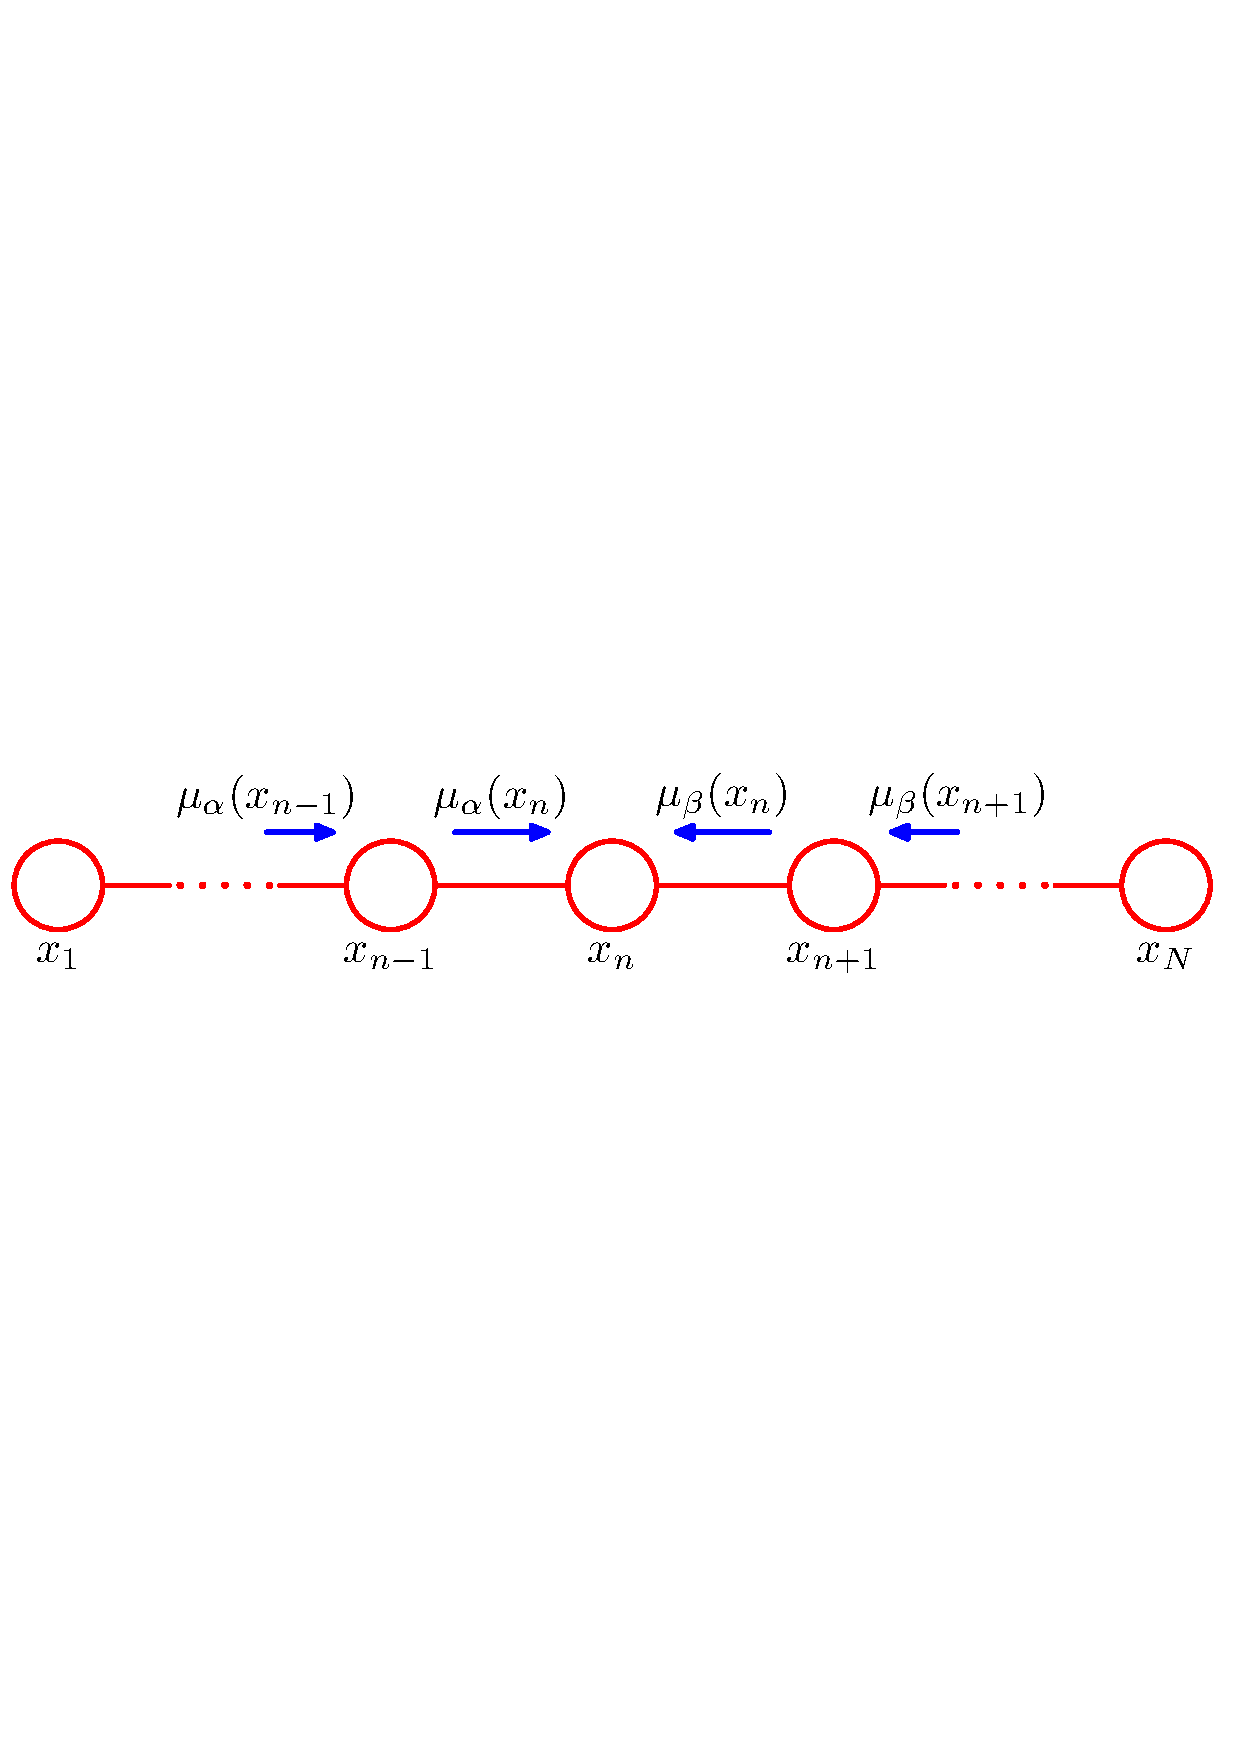
\includegraphics[width=0.5\textwidth]{figures/graphical_models_sum_product_message_passing.pdf}
		\caption{Message passing in graphical models (Bishop 8.38)}
	\end{figure}
	\item Even the normalization term $Z$ can be expressed by the messages: $Z=\sum_{x_n}\mu_{\alpha}(x_n)\mu_{\beta}(x_n)$
	\item The benefit of this recursive implementation is that we don't have to take a sum over $d$ variables ($\mathcal{O}(K^{d})$), but only have to take sums over two variables at a time ($\mathcal{O}(K^{2}d)$). Hence, the computational time scales linear with number of nodes instead exponential.
	
	Furthermore, we can share calculations between nodes, as the same messages can be re-used. Thus, calculating the marginals for all variables reduces to $\mathcal{O}(2\cdot K^2{d})=\mathcal{O}(K^2{d})$
\end{itemize}
\subsubsection{Sum-product algorithm}
\begin{itemize}
	\item The message passing idea is not limited to a Markov chain, but can be applied to any graph. For simplicity, we focus here on \textit{trees}, i.e. graphs where all nodes are connected, but without any loops/cycles, independent of the direction of the edges.
	\item In our discussion, we will focus on factor graphs as they represent the most general form of graphical models. Furthermore, cycles in MRFs can often be resolved in a factor graph so that we have less problem getting a tree-structured graph
	\item Now we will send messages from variables to factors, and from factors to variables. As a result, we get the marginalization for all variables. This algorithm is called \textbf{sum-product} algorithm as we only take sums and products
	\begin{figure}[ht!]
		\centering
		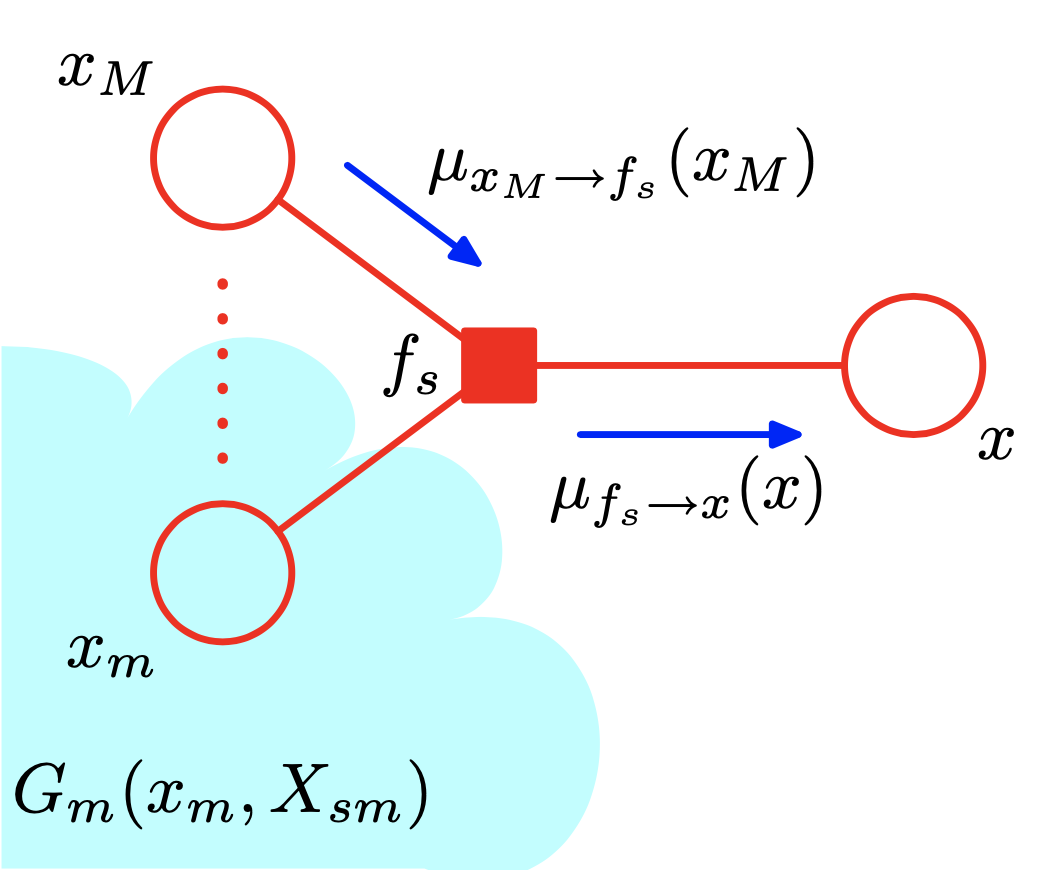
\includegraphics[width=0.2\textwidth]{figures/graphical_models_sum_product_messages_factor.png}
		\caption{Message passing to and from a factor node (Bishop 8.47)}
	\end{figure}
	\item The messages can be calculated as follows where we start at leaf nodes, and recursively go to the center of the tree:
	\begin{equation*}
	\tcbox[nobeforeafter]{\(
		\begin{split}
			\textbf{Factor$\to$Variable:} & \hspace{2mm} \mu_{\alpha\to i}(x_i)=\sum_{\bm{x}_{\alpha}} f_{\alpha}(\bm{x}_{\alpha})\prod_{j\in \alpha\setminus i}\mu_{j\to\alpha}(x_j)\\
			& \text{If $\alpha$ leaf node:} \hspace{2mm}\mu_{\alpha\to i}(x_i)=\sum_{\bm{x}_{\alpha}} f_{\alpha}(\bm{x}_{\alpha})\\
			\textbf{Variable$\to$Factor:} & \hspace{2mm} \mu_{j\to \alpha}(x_j)=\prod_{\beta\in \text{ne}(j)\setminus \alpha}\mu_{\beta\to j}(x_j)\\
			&\text{If $j$ leaf node:} \hspace{2mm}\mu_{j\to \alpha}(x_j)=1
		\end{split}
		\)}
	\end{equation*}
	The marginalizations/beliefs are in the end:
	\begin{equation*}
	\tcbox[nobeforeafter]{\(
		\begin{split}
		\textbf{Variable belief:} & \hspace{2mm} p(x_i)=\frac{1}{Z}\prod_{\alpha\in\text{ne}(i)}\mu_{\alpha\to i}(x_i)\hspace{5mm}\text{where}\hspace{2mm}Z=\sum_{x_i}\prod_{\alpha\in\text{ne}(i)}\mu_{\alpha\to i}(x_i)\\
		\textbf{Factor belief:} & \hspace{2mm} p(\bm{x}_{\alpha})=\frac{1}{Z}f_{\alpha}(\bm{x}_\alpha) \prod_{i \in\text{ne}(\alpha)}\mu_{i \to\alpha}(x_i)\\
		\end{split}
		\)}
	\end{equation*}
	where a factor belief is the marginalization of all variables except those with an direct edge to the factor.
	\item The complexity of this algorithm scales with $\mathcal{O}(EK^{M})$ where $E$ are the number of edges, $M$ the maximum number of variables that are connected to a factor, and $K$ the maximum domain size
	\item Note that this algorithm is only exact on trees or forest (group of trees). For general graphs, we can first bring them into the shape of a tree by e.g. \textbf{variable elimination}
	\begin{itemize}
		\item Given a MRF or factor graph, we will marginalize out these variable nodes which cause a loop in our graphical model. Let's for example consider this model:
		\begin{figure}[ht!]
			\centering
			\tikz{ %
				\node[latent] (xA) {$X_A$} ; %
				\node[latent, right=of xA] (xB) {$X_B$} ; %
				\node[latent, below=of xA] (xC) {$X_C$} ; %
				\node[latent, right=of xC] (xD) {$X_D$} ; %
				\node[latent, right=of xD] (xE) {$X_E$} ; %
				
				\edge[-]{xA}{xB};
				\edge[-]{xB}{xD};
				\edge[-]{xC}{xD};
				\edge[-]{xE}{xD};
				\edge[-]{xE}{xB};
			}
		\end{figure}
		\item We can do this by simply writing down the joint probability distribution and determine a order of variables $X_1,...,X_M$ where the last variables, e.g. $X_M$, should be those which are eliminated (likely the easiest to marginalize). We then sort the sums according to the selected order.
		
		In our example, we want to eliminate $X_E$ as it has the least connections from those in the loop. The sum order is therefore:
		\begin{equation*}
			\hspace{-10mm}p(X_A,...,X_E) = \frac{1}{Z}\sum_{X_B}\sum_{X_A} \psi_{A,B}(X_A, X_B)\sum_{X_D}\psi_{B,D}(X_B, X_D) \sum_{X_C}\psi_{C,D}(X_C, X_D)\sum_{X_E} \psi_{B,E}(X_B, X_E)\psi_{D,E}(X_D, X_E)
		\end{equation*}
		\item Finally, replace the marginalized terms by a new factor, and remove node from graph. In the example, we would replace $\tau(X_B, X_D) = \sum_{X_E} \psi_{B,E}(X_B, X_E)\psi_{D,E}(X_D, X_E)$. This can be merged into the potential $\psi_{B,D}$, hence not changing the graph structure. Our final graph is a tree again, and looks as follows:
		\begin{figure}[ht!]
			\centering
			\tikz{ %
				\node[latent] (xA) {$X_A$} ; %
				\node[latent, right=of xA] (xB) {$X_B$} ; %
				\node[latent, below=of xA] (xC) {$X_C$} ; %
				\node[latent, right=of xC] (xD) {$X_D$} ; %
				
				\edge[-]{xA}{xB};
				\edge[-]{xB}{xD};
				\edge[-]{xC}{xD};
			}
		\end{figure}
	\end{itemize}
	\item The sum-product algorithm so far only calculated marginals. To set some observed variables as observed, we can use the same algorithm, but simply add additional ``hard evidence'' factor nodes, which is nothing else than a hard prior that $x_j$ has the value $\xi_j$:
	$$f_{\xi_j}(x_j)=\delta(x_j=\xi_j)$$
	Then if we apply the sum product algorithm on the extended graph again, we get the conditionals $p(x_i|x_j=\xi_j)$
\end{itemize}
\subsubsection{Max-sum algorithm}
\begin{itemize}
	\item The sum-product algorithm calculates the full marginal distribution $p(x_j)$, but sometimes, we just want to know the most likely value of $x_j$, especially if we set some variables to observed states
	\item As it turns out, we can use a very similar algorithm for this, but simply replace sums by maximum operators, and products by sums.
	\item First, let's consider what the optimum is in the general case:
	$$\bm{x}^{*}=\arg\max_{\bm{x}} \prod_{\alpha} f_{\alpha}(\bm{x}_{\alpha})$$
	where we can ignore the normalization constant. Furthermore, to simplify optimization, we can apply the log:
	$$\bm{x}^{*} = \arg\max_{\bm{x}} \sum_{\alpha} \ln f_{\alpha}(\bm{x}_{\alpha})$$
	\item Our messages passed across the graph are then as follows:
	\begin{equation*}
	\tcbox[nobeforeafter]{\(
		\begin{split}
		\textbf{Factor$\to$Variable:} & \hspace{2mm} \nu_{\alpha\to i}(x_i)=\max_{\bm{x}_{\alpha\setminus i}} \log f_{\alpha}(\bm{x}_{\alpha}) + \sum_{j\in \alpha\setminus i}\nu_{j\to\alpha}(x_j)\\
		& \text{If $\alpha$ leaf node:} \hspace{2mm}\nu_{\alpha\to i}(x_i)=\max_{\bm{x}_{\alpha\setminus i}} f_{\alpha}(\bm{x}_{\alpha})\\
		\textbf{Variable$\to$Factor:} & \hspace{2mm} \nu_{j\to \alpha}(x_j)=\sum_{\beta\in \text{ne}(j)\setminus \alpha}\nu_{\beta\to j}(x_j)\\
		&\text{If $j$ leaf node:} \hspace{2mm}\nu_{j\to \alpha}(x_j)=0
		\end{split}
		\)}
	\end{equation*}
	\item The maximum beliefs/marginals are:
	\begin{equation*}
	\tcbox[nobeforeafter]{\(
		\begin{split}
		\textbf{Max-marginals:} & \hspace{2mm} q_i(x_i)=\sum_{\alpha\in\text{ne}(i)}\nu_{\alpha\to i}(x_i)\\
		\end{split}
		\)}
	\end{equation*}
	\item In the case that $q_i(x_i)$ has a unique maximum, we can simply take the argmax to get the optimum: $x^{*}_i = \arg\max_{x_i} q_i(x_i)$
	
	If this is not the case, we need to run the Viterbi algorithm (Bishop 8.4.5, we do not go in detail for this in the exam) to get the global optimum. The general idea is that some optima might depend on each other. For example, if we have something similar to a XOR, $(x_0=0, x_1=1)$ and $(x_0=1,x_1=0)$ are the optimums, but just looking at the independent marginals, $(x_0=0,x_1=0)$ and $(x_0=1,x_1=1)$ would be also optima. We can prevent this by slightly extending the messages passed around.
\end{itemize}